\begin{adjustwidth*}{}{-2.25in}
\textbf{{\large Exercises}}
\setlength{\columnsep}{25pt}
\begin{multicols*}{2}
\noindent Terms and Concepts \small
\begin{enumerate}[1)]
\item Define the term ``antiderivative'' in your own words.
\item Is it more accurate to refer to ``the'' antiderivative of $f(x)$ or ``an'' antiderivative of $f(x)$?
\item Use your own words to define the indefinite integral of $f(x)$.
\item Fill in the blanks: ``Inverse operations do the \underline{\hskip .5in} things in the \underline{\hskip .5in} order.''
\item The derivative of a position function is a \underline{\hskip .5in} function.
\item The antiderivative of an acceleration function is a \underline{\hskip .5in} function.
\item How are definite and indefinite integrals related?
\item What constant of integration is most commonly used when evaluating definite integrals?
\item The definite integral can be used to find ``the area under a curve.'' Give two other uses for definite integrals.
\end{enumerate} 

\noindent {\normalsize Problems} \small

\noindent{\bf In exercises 4--27, evaluate the indefinite integral.}

\bmtwo
\begin{enumerate}[1),resume]
\item $\ds \int 3x^3\ dx$
\item $\ds \int x^8\ dx$
\item $\ds \int (10x^2-2)\ dx$
\item $\ds \int  dt$
\item $\ds \int 1\  ds$
\item $\ds \int \frac{1}{3t^2}\  dt$
\item $\ds \int \frac{3}{t^2}\  dt$
\item $\ds \int \frac{1}{\sqrt{x}}\  dx$
\item $\ds \int \sec^2(\theta)\  d\theta$
\item $\ds \int \sin(\theta)\  d\theta$
\item $\ds \int 5e^\theta\  d\theta$
\item $\ds \int 3^t\  dt$
\item $\ds \int \frac{5^t}{2}\  dt$
\item $\ds \int (2t+3)^2\  dt$
\item $\ds \int (t^2+3)(t^3-2t)\  dt$
\item $\ds \int x^2x^3\  dx$
\item $\ds \int e^\pi\  dx$
\item $\ds \int t\  dx$
\end{enumerate}
\emtwo

\noindent{\bf In exercises 28--38, solve the initial value problem.}

\begin{enumerate}[1),start=28]
\item $\fp(x) = \sin (x)$ and $f(0)= 2$
\item $\fp(x) = 5e^x$ and $f(0)= 10$
\item $\fp(x) = 4x^3-3x^2$ and $f(-1)= 9$
\item $\fp(x) = \sec^2 (x)$ and $f(\pi/4)= 5$
\item $\fp(x) = 7^x$ and $f(2)= 1$
\item $\fpp(x) = 5$ and $\fp(0)= 7$, $f(0) = 3$
\item $\fpp(x) = 7x$ and $\fp(1)= -1$, $f(1) = 10$
\item $\fpp(x) = 5e^x$ and $\fp(0)= 3$, $f(0) = 5$
\item $\fpp(x) = \sin (\theta)$ and $\fp(\pi)= 2$, $f(\pi) = 4$
\item $\fpp(x) = 24x^2+2^x-\cos (x)$ and $\fp(0)= 5$, $f(0) = 0$
\item $\fpp(x) = 0$ and $\fp(1)= 3$, $f(1) = 1$
\end{enumerate}

\noindent{\bf In exercises 39--51, evaluate the definite integral.}

\bmtwo
\begin{enumerate}[1),resume]
\item $\ds\int_1^3 (3x^2-2x+1)\ dx$
\item $\ds\int_0^4 (x-1)^2\ dx$
\item $\ds\int_{-1}^1 (x^3-x^5)\ dx$
\item $\ds\int_{\pi/2}^\pi \cos (x)\ dx$
\item $\ds\int_{0}^{\pi/4} \sec^2 (x)\ dx$
\item $\ds\int_{1}^{e} \frac1x \ dx$
\item $\ds\int_{-1}^{1} 5^x \ dx$
\item $\ds\int_{-2}^{-1} (4-2x^3) \ dx$
\item $\ds\int_{1}^{3} e^x \ dx$
\item $\ds\int_{0}^{4} \sqrt{t} \ dt$
\item $\ds\int_{9}^{25} \frac{1}{\sqrt{t}} \ dt$
\item $\ds\int_{1}^{8} \sqrt[3]{x} \ dx$
\item $\ds\int_{1}^{2} \frac1{x} \ dx$
\item $\ds\int_{1}^{2} \frac1{x^2} \ dx$
\item $\ds\int_{1}^{2} \frac1{x^3} \ dx$
\item $\ds\int_{0}^{1} x \ dx$
\item $\ds\int_{0}^{1} x^2 \ dx$
\item $\ds\int_{0}^{1} x^3 \ dx$
\item $\ds\int_{0}^{1} x^{100} \ dx$
\item $\ds\int_{-4}^{4} \ dx$
\item $\ds\int_{-10}^{-5} 3\ dx$
\item $\ds\int_{-2}^{2} 0\ dx$
\item $\ds \int_{\pi/6}^{\pi/3} \csc (x)\cot (x)\ dx$
\end{enumerate}
\emtwo

\begin{enumerate}[1),start=62]
\item $\ds\int_{0}^{\pi} (2\cos (x) - 2\sin (x)) \ dx$
\item Explain why:
\begin{enumerate}
\item		$\ds \int_{-1}^1 x^n\ dx=0$, when $n$ is a positive, odd integer, and 
\item		$\ds \int_{-1}^1 x^n\ dx = 2\int_{0}^1 x^n\ dx$ when $n$ is a positive, even integer.
\end{enumerate}
\end{enumerate}

\noindent{\bf In exercises 64--68, a velocity function of an object moving along a straight line is given. Find the displacement of the object over the given time interval.}

\begin{enumerate}[1),resume]
\item $v(t) = -32t+20$ ft/s on $[0,5]$
\item $v(t) = -32t+200$ ft/s on $[0,10]$
\item $v(t) = 2^t$ mph on $[-1,1]$
\item $v(t) = \cos (t)$ ft/s on $[0,3\pi/2]$
\item $v(t) = \sqrt[4]{t}$ ft/s on $[0,16]$
\end{enumerate}

%------------------------------------------
% END OF EXERCISES ON FIRST PAGE
%------------------------------------------
\end{multicols*}
\end{adjustwidth*}

\clearpage

\begin{adjustwidth*}{}{-2.25in}
\setlength{\columnsep}{25pt}
\begin{multicols*}{2}\small

\noindent{\bf In Exercises 69--72, an acceleration function of an object moving along a straight line is given. Find the change of the object's velocity over the given time interval.}

\begin{enumerate}[1),start=69]
\item $a(t) = -32$ ft/s$^2$ on $[0,2]$
\item $a(t) = 10$ ft/s$^2$ on $[0,5]$
\item $a(t) = t$ ft/s$^2$ on $[0,2]$
\item $a(t) = \cos (t)$ ft/s$^2$ on $[0,\pi]$

    \item A function $f$ is given piecewise by the formula
  $$f(x) = \left\{ 
  	\begin{array}{lr}
	-x^2 + 2x + 1, & \ \mbox{if} \ 0 \le x < 2 \\
	-x + 3, & \ \mbox{if} \ 2 \le x < 3 \\
	x^2 - 8x + 15, & \ \mbox{if} \ 3 \le x \le 5
	\end{array}
	\right.
  $$
  \ba
  	\item Determine the exact value of the net signed area enclosed by $f$ and the $x$-axis on the interval $[2,5]$.
	\item Compute the exact average value of $f$ on $[0,5]$.
	\item Find a formula for a function $g$ on $5 \le x \le 7$ so that if we extend the above definition of $f$ so that $f(x) = g(x)$ if $5 \le x \le 7$, it follows that $\int_0^7 f(x) \, dx = 0.$
  \ea
\end{enumerate}

\begin{enumerate}[1),resume]
 \item The instantaneous velocity (in meters per minute) of a moving object is given by the function $v$ as pictured below.  Assume that on the interval $0 \le t \le 4$, $v(t)$ is given by $v(t) = -\frac{1}{4}t^3 + \frac{3}{2}t^2 + 1$, and that on every other interval $v$ is piecewise linear, as shown.

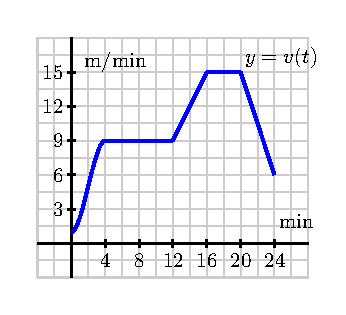
\includegraphics[scale=.75]{figures/4_4_Ez2.eps}

    \ba
  	\item Determine the exact distance traveled by the object on the time interval $0 \le t \le 4$.
	\item What is the object's average velocity on $[12,24]$?
	\item At what time is the object's acceleration greatest?
	\item Suppose that the velocity of the object is increased by a constant value $c$ for all values of $t$.  What value of $c$ will make the object's total distance traveled on $[12,24]$ be $210$ meters?
  \ea
  
    \item When an aircraft attempts to climb as rapidly as
possible, its climb rate (in feet per minute) decreases as altitude
increases, because the air is less dense at higher altitudes.
Given below is a table showing performance data for a certain
single engine aircraft, giving its climb rate at various altitudes, where  $c(h)$ denotes the climb rate of the airplane at an altitude $h$.


\begin{center}
\scalebox{.85}{
  \begin{tabular}{|c||c|c|c|c|c|c|}
    \hline
    $h$ (feet)& $0$ & $1000$ & $2000$ & $3000$ & $4000$ & $5000$\\
    \hline
    $c$ (ft/min)& $925$ & $875$ & $830$ & $780$ & $730$ & $685$\\
    \hline
    \hline
    $h$ (feet)& $6000$ & $7000$ & $8000$ & $9000$ & $10,000$ &\\
    \hline
    $c$ (ft/min)& $635$ & $585$ & $535$ & $490$ & $440$ &\\
    \hline
  \end{tabular}
  }
\end{center}


 Let a new function called $m(h)$ measure
the number of minutes required for a plane at altitude $h$ to climb the
next foot of altitude.
\ba
	\item Determine a similar table of values for $m(h)$ and explain how it is related to the table above.  Be sure to explain the units.

	\item Give a careful interpretation of a function whose derivative
is $m(h)$.  Describe what the input is and what the output is.  Also,
explain in plain English what the function tells us.

	\item Determine a definite integral whose value tells us exactly the number of minutes required for the airplane to ascend to
$10,000$ feet of altitude.  Clearly explain why the value of this integral has the required meaning.

	\item Use the Riemann sum $M_5$ to estimate the value of the integral you found in (c).  Include units on your result.
\ea


\end{enumerate}

%---------------------------------------------
% END OF EXERCISES ON SECOND PAGE
%---------------------------------------------
\end{multicols*}
\end{adjustwidth*}

\afterexercises